%\section{Implementation}
This chapter is dedicated to the implementation of the presented system. In this chapter we will explain in detail what has been implemented and how. 

\section{System}
The system has been implemented using Java and Servlets for the back-end, and JSP and Javascript for displaying the webpages in the front-end. We have chosen to use MySQL as a database since it is known to all the members. The database is used to store the policy entities (the policy entity is explained in subsection \ref{s:Domain}). There is also a logging subsystem that is used to create logs about the system and its execution. This has been implemented using the log4j library and it creates a log file which contains all the logged data. 
\\The back-end deals with requests from the front-end and executes at a specific time interval, the active policies at that time. The front-end displays the policies and enables the creation, modification or deletion of policies. However, because we have chosen to serialize the policies to JSON, in the frontend these policies have to be deserialised and parsed to be displayed properly. 
\\A serialized policy to JSON has the following structure (see Figure \ref{fig:json_policy})
It contains a statement object which is composed of the objects conditionalExpressions, thenStatements and elseStatements. 
The conditional expressions describe the IfStatements and has information about the sensor id, the prefix operator, and the operator. The thenStatements and elseStatements express the desired value of the sensor id. 

\begin{figure}
	\centering
    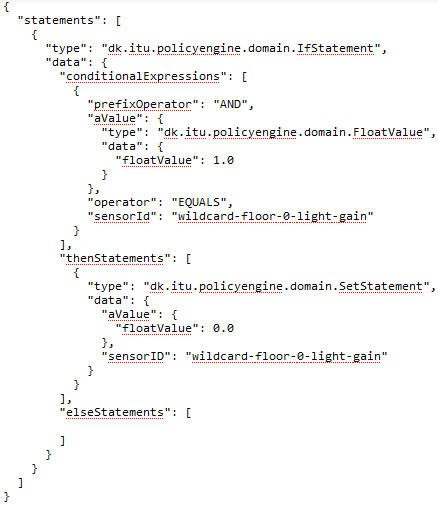
\includegraphics[scale=0.85]{images/json_policy.png} 
	\caption{A serialized policy}
	\label{fig:json_policy}
\end{figure}

\subsection{Interfaces}
There are two interfaces that describe the methods of Statements and Value classes. Each statement should implement an execute method, in which specific execution is done. 
\subsection{Domain}
\label{s:Domain}
\begin{figure}
	\centering
    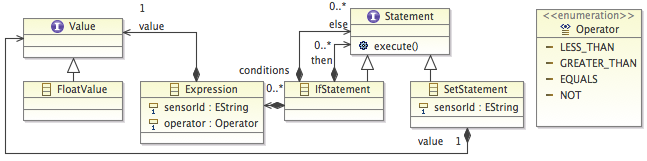
\includegraphics[scale=0.55]{chapters/implementation-model-expression-language.png} 
	\caption{The core classes in the \textit{expression language}.}
	\label{fig:ecore-sensors-actuators}
\end{figure}

A statement can either be a SetStatement or an IfStatement. The SetStatement sets an value in the building server (in effect it is an actuator). It is possible to have nested IfStatements, making the policies both flexible and simple. An IfStatement can contain multiple expressions that all are being anded when evaluated. If the user wants to make an IfStatement with or between the expressions, will have to use a nested IF. The optimal solution to this would be to make a safe left-recursive model. We did not have enough time for this, but we will elaborate further on this subject in the \nameref{chapter:discussion} section. 

An Expression has three variables, the sensorId, the operator and a value of type Value. When the policy engine is running, each expression is being evaluated. The current value of the sensor is fetched and compared to the desired value using the operator. An expression can contain the following operators; <, >, <=, >=, !=,=. 
If the evaluation of the expression is true, then the statement is executed.

The FloatValue class implements the Value interface and it represents a value of type float. This is used to set the values of the sensors, as those can be of float type. However, at this moment we only support to set integer values, 1 for On and 0 for Off.

A Policy object consists of statements and the policy can be run by executing those statements. A PolicyEntity object holds a policy and different properties of that policy such as name, description, interval, id and active. The interval property defines from which time to which time should the policy be enforced to run. This is implemented as a separate class, Interval, because of the serialization logics.  The active property represents the status of the policy as in if the user wishes for this policy to be executed (active) or not (not active).

To be able to handle many sensors and actuators, we have implemented Wildcards which define the sensors and actuators handled, and their type property (gain,setpoint). An example of a wildcard is "wildcard-floor-0-light-gain". This expresses that we want to retrieve to work on the gain of the light sensors from the floor 0. 
\section{Persistence}
We have decided to have our policies stored in a database as we think it is better to have them on a different server than the one running our policy engine. This may be a drawback if the The database chosen was MySQL as it is well known and used by the group. Because we do not have a complex persistence system, we decided to use the simple JDBC for connecting and querying the database, and not use other specialized frameworks such as Hibernate. 
\\Methods for communicating with the database are defined in the DataAccessLayer class. There are the methods for creating, reading, updating and deleting policies. In addition, it is of great interest to have a method that returns only the policies that are running at the current time and are active. 
\\Because the fact that different policies may operate on the same sensors, we decided to use a cache to store each sensor's value. This reduces the number of queries to the building server so it does not crash. This cache is implemented using a hashtable and stores the value of the sensor. After executing all the active policies at that moment, this cache is cleared. 
\section{Building querying}
To communicate with the building's server, we created the Connection class which provides methods for connecting to it and parses the JSON object received. There are several methods implemented that parse the response of the server and offer information such as - a list with the sensors in a room by providing the room id, a list with all the sensors of a certain type (e.g ac, light, heater etc.) The two most important methods are for retrieving the sensor's value and setting it to a specific one. 

\begin{figure}
	\centering
    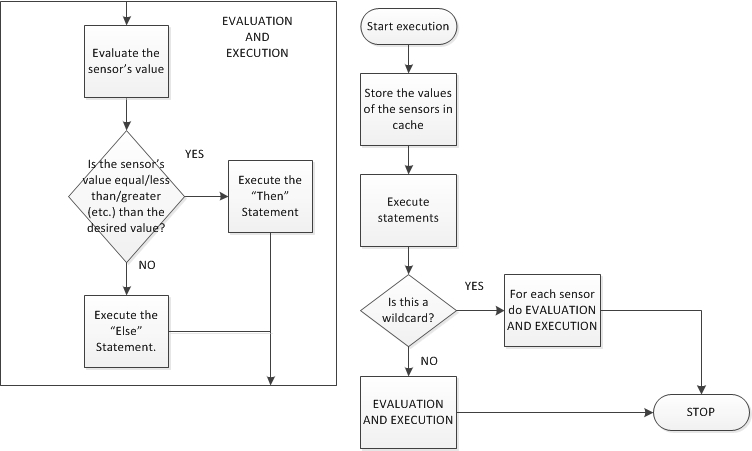
\includegraphics[scale=0.65]{images/policy_execution_flow.png} 
	\caption{The execution flow of a policy.}
	\label{fig:policy_execution_workflow}
\end{figure}

To retrieve a sensor's value we use the GetSensorValue method which takes as argument the sensor id, and returns a String with the value. By default, the last value sorted by timestamp that exists is returned.  
\\ To set a value we use the method SetSensorValue which takes as parameters the sensor's id and the value we want to set. 
\section{Executing policies} 
The system executes the active policies at a specific time interval. This execution has the following flow \ref{fig:policy_execution_workflow}:
First, a list with the active policies at that time is retrieved. Then the statements that compose the policy are retrieved along with their expressions. In these expressions resides the sensor id on which operations will occur next. For each sensor it is retrieved its last value from the building api and stored in the cache. After storing all the values of the sensors, the statements are executed. 
\\The first statements that are executed are the IfStatements. Here a check if the policy is a wildcard is done.  If it is a wildcard, then the statements are executed for each sensor by evaluating its value against the desired value. If the evaluation returns false, then the else statements are executed. If the policy is not a wildcard, an evaluation of the sensor's value it's done and depending on its result, the then statementes or else statements are executed. 
In the evaluation part the actual value of the sensor is compared to the desired value using the operator defined in the expression. This evaluation returns true or false and so execution of the thenStatements is done if the evaluation is true otherwise the elseStatements are executed.
In the execution of the then and else statements, the new sensor value is set in the server. 